%%% Data and Methodology
%%%%%%% Wording: ⏳
%%%%%%% Styling: ⏳
%%%%%%% References: ⏳
%%%%% Grammar: ⏳
%%% --------------------------------------------------------------
\chapter{Data and Methodology}
\label{ch:data-methodology}
This chapter addresses the process and challenges of local environment setup, obtaining, preparing and anonymizing the data.
Most importantly, this chapter describes and explains the data that was used for this research.
It also briefly describes the tools, technologies and methods employed to answer the research questions.


\section{Environment and local setup}
\label{sec:data-methodology-environment}

To start off, we needed to set up some kind of environment where we would later work with the data.
The data we would be working with was stored in a PostgreSQL database.

Having direct access to the production database to perform the analysis was not a secure and ethical way to go.
Exporting only the necessary and raw data from the production database was an initial thought, but we initially did not know what data we would need, and by exporting we would lose all the relations between the tables.

Therefore, we decided to set up a local database with the same structure as the production database where we can query and analyze the data safely.
The next step was to import the data from the production database to the local database.
Importing or simple cloning the full database was also not an option, because only a small fraction of its subset was required.

So a deep internal analysis of the tables that were relevant to our study was performed.
This resulted in a list of total 21 tables that held the necessary data for the study and were necessary to be imported.

\subsection{Data Obtaining and Preparation}
\label{subsec:data-methodology-obtaining-preparation}

Almost every table was easily queried for the event and exported from the production database to a local CSV file.
But some tables (for example and not surprisingly, the \textit{transactions} table with over 140k rows) were too large to be exported in one piece, so we had to split them into smaller parts.
Later, these parts were joined together to a single CSV file using a simple Python script.

Since no direct access to the production database was used for the export but rather a database management tool, the export was not as fast as it could be and took a significant amount of time.
Moreover, the exported data, most importantly the timestamps, were in a different format than we needed.
And also all numeric values were exported as a formatted strings with a comma as a decimal separator.
So a data preprocessing Python script was written to convert such invalid columns to the correct format.

\subsection{Local Database Setup}
\label{subsec:data-methodology-local-database-setup}
Then a step to set up the local PostgreSQL database was needed.
Due to the nature of this study, we wanted to keep the setup as simple as possible, so we used the default PostgreSQL installation without using any special environment using Docker or similar.
However, during this process I made a mistake and forgot that a PostgreSQL with PostGIS extension was needed.
So it required to re-set up the database with the PostGIS extension.

The next step was to import the data from the CSV files to the local database.
For further database handling, analysis and visualization, we used DataSpell, a Python IDE with a built-in database explorer and data visualization tools.
DataSpell was then used for the local database import, which prior to it required some necessary database relations and constraints modifications, since the data was exported without them and was not relevant for the study.

This whole process resulted in approximately 387k rows of data in the local database that were ready to be queried and analyzed.

\subsection{Local Database Modifications}
\label{subsec:data-methodology-local-database-modifications}
Before any analysis was performed, some modifications to the local database were needed due to some known limitations and missing data.

\subsubsection{Beverage Volumes}
\label{subsubsec:data-methodology-local-database-modifications-volume}
The first necessary limitation that the Beverage Consumption Analysis section heavily relied on was the missing information about beverage products volume in milliliters.
This information was crucial for the analysis, so a new column was added to the relevant product information tables.
However, the next step was to back-fill this information which was not easily automated.

The First approach was to write a Python script that would try to find the volume information from the product name.
This worked for some products, but not for all since the naming convention was not consistent.

After several attempts to automate this process, it was decided to manually fill in the missing information since only 425 products were present in the database.
Only 159 of them were of beverage type and thus eligible for the volume information.

\subsubsection{Returnable Products}
\label{subsubsec:data-methodology-local-database-modifications-returnable}
Since one of the research questions was to analyze the returnable cups and this information was not easily available in the database, a new column was added to the product information tables.

This was a simple binary column that indicated whether the product was returnable or not.
Back-filling this information was also pretty straightforward since only one product was a returnable cup.

\subsubsection{Venue Map Visualization}
\label{subsubsec:data-methodology-local-database-modifications-venue-map}
One of the initial ideas was to visualize the venue map with the locations of the selling places, top-up service points, stages and other important places.

This would be invaluable, the database was partially ready for this, but the data would be significantly time-consuming to back-fill and the later analysis and visualization would require more time.

Since these facts and the fast that this process of preparing the data took place before completing the list of data analysis questions, this idea was later abandoned.

\subsubsection{Event Program}
\label{subsubsec:data-methodology-local-database-modifications-program}
To present some time-related data and its correlation with the event program, it would require to have the event program in the database.

Again, the database was ready for this, but no event program was set up, since it was unnecessary for the event.
Therefore, this required getting the event program from the festival website and manually insert it into the database.

This was manually a very time-consuming process, but it was necessary for the analysis.
For some simplification of the process, an AI tool was used to extract the data from the program schedule screenshots and instructed to prepare an SQL script that would insert the data into the database.

This seemed like a good idea, but the AI tool was initially hallucinating and made up some incorrect data.
But after several iterations, it successfully extracted the data and prepared the SQL script which was used and the event program was successfully inserted into the database.

In the end, I doubt that this process was faster than manual data entry, but it was a good exercise and a good example of how AI can be used to automate some processes.


\section{Data Anonymization}
\label{sec:data-methodology-anonymization}
The Data Anonymization process was necessary due to requirements initially set by the data provider and later by the ethical considerations.
This step was performed for the already imported data in the local database.
It required identifying the sensitive data and replacing them with anonymized values.

In this case, the most sensitive data were:
\begin{itemize}
	\item \textbf{Vendor names}: Since it included the legal names of the vendors, it was necessary to anonymize them.
	\item \textbf{Selling places}: Some selling places were named after the vendors, so it was necessary to anonymize them as well.
	\item \textbf{Customer information}: Some tables included customer information like names, emails, phone numbers, etc.
\end{itemize}

The process could have been done various ways, but the fact that this study will not be exposing internal database structure, it was decided to perform the anonymization directly in the database.

However, if one-way anonymization were to be performed, it would permanently overwrite the original data, losing the possibility to switch from anonymized to original data.
Therefore, a two-way anonymization process was chosen and performed.

This was particularly useful during the analysis phase, where the results would contain the original data for better understanding, fact-checking and for the internal presentation and consultations with the organizer.

It was done on the database level, where two new internal tables were introduced~–~\textit{public.anonymization\_config} and \textit{public.original\_values}.

Where the \textit{public.anonymization\_config} table held the configuration about which schema, table and column should be anonymized and how.
For the usage, a simple SQL function was created to define the anonymization configuration in a simple JSON format, that looked like in the~\fullref{lst:anonymization-configuration}.

\begin{listing}[H]
	\begin{minted}{sql}
		SELECT configure_anonymization('[
			{ "table": "schema.seller", "columns": ["legal_name", "name_int", "name_pub"] },
			...
			{ "table": "schema.user_account", "columns": ["email", "last_name", "first_name", "phone"] },
			]'::JSONB
		);
	\end{minted}
	\caption{Anonymization configuration example.}
	\label{lst:anonymization-configuration}
\end{listing}

The \textit{public.original\_values} table was used to store the original values of the anonymized columns.
Again, using a simple SQL function \textit{anonymize\_database()}, it would store the original values and anonymize the configured table columns.

One particular challenge was anonymizing the values smartly.
It could have been easily done by replacing the values with random strings, hashes or encrypted values.
But working with data, where a vendor is named \textit{fa65165b923e9cc} is not very convenient.

Therefore, a simple SQL function was written to anonymize the value depending on the configuration.
This allowed to configure the anonymization to:
\begin{itemize}
	\item replace vendor names with values like \textit{Vendor 1},
	\item customer emails with \textit{03b09592-d0eb-43a3-9941-30d38ade6bce@gmail.com} keeping the original email domain,
	\item selling places with values like \textit{Place 1} where the original name contained sensitive information, but keep original values for places like \textit{BAR L2},~etc.
\end{itemize}

In the end, it resulted in a database with anonymized values per stated configuration, that could have been used for the analysis and results presentation safely.
However, the original values were still present in the database, and the database could have been anytime easily restored to the original state if needed and vice versa.


\section{Data Structure}
\label{sec:data-methodology-structure}
Without exposing the internal database structure, the abstract data structure this study was working with can be described as follows:

\subsection{Financial Data}
\label{subsec:data-methodology-structure-financial}
\textbf{Transactions} (approx.\ 300k rows): Transactional data, that holds the information about the type, amount, timestamps and links to products, places and other related entities.
This analysis relies on and works with several transaction types, including \textbf{top-up charge} and \textbf{refund} transactions~\footnote{Top-up transactions mean funding or refunding chip credit balances.},
\textbf{order sales} and \textbf{refund} transactions~\footnote{Order transactions mean spending the credit balance for products.}~and
\textbf{chip registrations}\footnote{Chip registrations mean records of when the chip bracelets were registered by the system.}.

\textbf{Credit Refunds} (approx.\ 15k rows): Post-event credit refund requested by the customers with the information about the amount, timestamp, customer and the bank account to which the refund was sent.
This data enables our analysis to correctly handle disposable credit balances, more information about the anonymous customers~\footnote{Anonymous customer essentially means a user without registered account.}~and their behavior.

\begin{blue-box}{Why is it important?}
	These records also form the backbone of the analysis, enabling insights into revenue, sales trends, and customer behavior.
\end{blue-box}

\subsection{Customer Data}
\label{subsec:data-methodology-structure-customer}

\textbf{User Accounts} (approx.\ 5k rows): Registered customer accounts with the information about the user and its potential online order history and other related information.

\textbf{Tickets and Orders} (approx.\ 30k rows): Information about the online sold tickets, its types, prices, timestamps, online order related information.

\begin{blue-box}{Why is it important?}
	With the above data, this analysis can work with more customer information supporting the customer behavior analysis, customer segmentation and other related analysis.
\end{blue-box}

\subsection{Event Data}
\label{subsec:data-methodology-structure-event}

\textbf{Places} (approx.\ 400 rows): Selling and top-up service points, zones for access control and its other relations.

\textbf{Products} (approx.\ 500 rows): Essentially a product catalog including the product name, price, category, volume, seller ownership and seller-organizer deal related links.

Important information about products is their supported categorization that will later be used for the sales analysis and can be seen in~\autoref{tab:product-categories}.

\begin{table}[H]
	\centering
	\footnotesize
	\begin{tabularx}{\textwidth}{|>{\columncolor{unicorn_blue!5}}X|>{\columncolor{unicorn_blue!5}}l|}
		\hline
		\rowcolor{unicorn_blue}
		\textbf{\color{white} Category} & \textbf{\color{white} Description}                                    \\
		\hline
		\hline
		Nonalcoholic                      & Any non-alcoholic beverages (e.g., coffee, water, etc.)               \\
		Beer                              & Any kind of beer.                                                     \\
		Wine                              & Any kind of wine.                                                     \\
		Other Alcohol                     & Any other kind of alcoholic beverages (e.g., shots, cocktails, etc.). \\
		Salty                             & Any salty snacks.                                                     \\
		Sweet                             & Any sweet snacks.                                                     \\
		Other                             & Any other products that do not fit into the above categories.         \\
		\hline
	\end{tabularx}
	\caption{Product categories}
	\label{tab:product-categories}
\end{table}

\textbf{Event Program} (approx.\ 140 rows): Event program schedule with the information about the stages, performers, times and other related information.

\begin{blue-box}{Why is it important?}
	This data provides more context to the event when combined with the financial and customer data above.
	Enabling the analysis to work with the event program, its correlation with the sales, customer behavior and other related analysis.
\end{blue-box}

\subsection{Data Processing Views}
\label{subsec:data-methodology-structure-views}
To efficiently query the studied data during the analysis, several SQL views and functions were created to simplify and speed up the process.

\textbf{Transaction Commission Calculation}: A function that calculates the commission for each transaction based on the product and the seller-organizer deal.
This was a crucial method required to calculate and analyze the commission from event order sales contributing to the organizer's revenue.

\textbf{Transaction Enrichment}: Since the transactional data consisted of several transaction types which were not easily distinguishable, a view was created to enrich the transaction data with the transaction type information.
It also benefited from the transaction commission calculation function mentioned above which helped to easily calculate the commission for each transaction.

\textbf{Chip Customers}: Probably the most complex function that returns the customers at the event.
Since the transactional data is architected using Event Sourcing, the customer information is not directly available and needs to be compiled from the transactional history.
This function was constructed in a way, where it supports time-based filtering and provides extensive insights into the customers, which is shown in~\autoref{tab:chip-customers-columns}~below:

\begin{table}[H]
	\centering
	\footnotesize
	\begin{tabularx}{\textwidth}{|>{\columncolor{unicorn_blue!5}}X|>{\columncolor{unicorn_blue!5}}l|}
		\hline
		\rowcolor{unicorn_blue}
		\textbf{\color{white} Column Name} & \textbf{\color{white} Description}                           \\
		\hline
		\hline
		CHIP\_ID                             & Unique chip identifier.                                      \\
		CHIP\_TYPE                           & Type of chip (\eg~regular, VIP, online, staff).              \\
		REG\_AT                              & Timestamp of chip registration.                              \\
		FIRST\_TRX                           & First transaction timestamp associated with the chip.        \\
		LAST\_TRX                            & Last transaction timestamp associated with the chip.         \\
		LAST\_BALANCE                        & Last known balance at the specified time frame.              \\
		ACTUAL\_BALANCE                      & Balance at the specified time frame after credit refunds.    \\
		\hline
		IS\_BLOCKED                          & Indicates if the chip is blocked due to suspicious activity. \\
		HOURS\_ACTIVE                        & Total active hours of the chip (daily sum).                  \\
		DAYS\_ACTIVE                         & Total number of days the chip was active.                    \\
		\hline
		T\_COUNT                             & Total number of transactions associated with the chip.       \\
		O\_TOTAL\_CNT                        & Total number of orders placed using the chip.                \\
		O\_TOTAL\_AMT                        & Total amount spent through orders.                           \\
		O\_MAX\_AMT                          & Maximum amount spent in a single order.                      \\
		O\_AVG\_AMT                          & Average amount spent per order.                              \\
		O\_MODE\_AMT                         & Most common amount spent per order.                          \\
		OS\_AVG\_AMT                         & Average amount spent on sales orders (excluding refunds).    \\
		OS\_MODE\_AMT                        & Most common sale amount (excluding refunds).                 \\
		TU\_TOTAL\_CNT                       & Total number of top-ups made to the chip.                    \\
		TU\_TOTAL\_AMT                       & Total amount credited to the chip via top-ups.               \\
		TU\_MAX\_AMT                         & Maximum amount credited in a single top-up.                  \\
		TU\_AVG\_AMT                         & Average amount credited per top-up.                          \\
		TU\_MODE\_AMT                        & Most common amount credited per top-up.                      \\
		TU\_CARD\_BRAND                      & Used card brand for top-ups (\eg~Visa, Mastercard).          \\
		\hline
		BR\_AMT                              & Total amount refunded to the customer's bank account.        \\
		BR\_EMAIL\_DOMAIN                    & Domain of the refund request email (\eg~gmail.com).          \\
		BR\_COUNTRY                          & Country associated with the bank account for refund.         \\
		BR\_REQ\_SOURCE                      & Source of the refund request (\eg~iOS, Android, Web).        \\
		BR\_BANK\_NAME                       & Name of the Czech bank used for the refund.                  \\
		BR\_CREATED                          & Timestamp when the refund request was created.               \\
		BR\_APPROVED                         & Timestamp when the refund request was approved.              \\
		\hline
		A\_EMAIL\_DOMAIN                     & Email domain of the account.                                 \\
		A\_COUNTRY\_NAME                     & Country associated with the account.                         \\
		A\_REQ\_SOURCE                       & Source of the account creation (\eg~iOS, Android, Web).      \\
		EO\_PAYMENT\_METHOD                  & Payment method for orders (\eg~card, bank transfer).         \\
		EO\_CARD\_BRAND                      & Used card brand for online order (Visa, Mastercard)          \\
		EO\_REQ\_SOURCE                      & Source of the order request (\eg~iOS, Android, Web).         \\
		\hline
	\end{tabularx}
	\caption{Customer chips function return table.}
	\label{tab:chip-customers-columns}
\end{table}

For further understanding, an enumeration of chip types should be mentioned; that can be seen in~\autoref{tab:chip-types}.

\begin{table}[H]
	\centering
	\footnotesize
	\begin{tabularx}{\textwidth}{|>{\columncolor{unicorn_blue!5}}X|>{\columncolor{unicorn_blue!5}}l|}
		\hline
		\rowcolor{unicorn_blue}
		\textbf{\color{white} Chip Type} & \textbf{\color{white} Description}                                 \\
		\hline
		\hline
		Regular                            & Chip issued at the event without any prior credit.                 \\
		VIP                                & VIP chip issued with artificial credit on behalf of the organizer. \\
		Online                             & Chip issued via online purchase or top-up                          \\
		Staff                              & Chip issued to the staff members.                                  \\
		Guest                              & Chip issued to the guests (band members, etc.)                     \\
		\hline
	\end{tabularx}
	\caption{Chip types enumeration}
	\label{tab:chip-types}
\end{table}


\section{Tools and Technologies}
\label{sec:data-methodology-tools}

As mentioned earlier, this process utilized a variety of tools and technologies to handle the data and prepare for the analysis.
These main tools and technologies included:
\begin{itemize}
	\item \textbf{PostgreSQL}: An open-source relational database management system used to store and query the data.
	\item \textbf{PostGIS}: An extension of PostgreSQL that supports geospatial data, enabling spatial analysis and visualization.
	\item \textbf{DataSpell}: An integrated development environment (IDE) for data science and analytics, used for database exploration and data visualization.
	\item \textbf{Python}: Used for data preprocessing, querying, and analysis, along with libraries like Pandas for data manipulation.
	\item \textbf{Claude AI}: Utilized for extracting data from unstructured sources (e.g., program schedules) and automating repetitive tasks like data entry.
\end{itemize}

Using such tools during this process provided a convenient environment for data handling and processing, initial analysis and ensuring the accuracy and efficiency for further analysis and results presentation.


\section{Conclusion}
\label{sec:data-methodology-conclusion}
This chapter laid out the process of setting up the local environment, collecting and preparing the data, anonymizing sensitive information and introducing the data structure.

Some key challenges, such as missing beverage volume information, data anonymization, and event program integration, were addressed through a combination of manual and automated processes.

In the end, the use of SQL views for data enrichment and functions for further data processing ensured efficient querying and analysis.
And hopefully laid the groundwork for answering the research questions and achieving the study's goals, as detailed in the later chapters.

For better understanding and visualization of this initial comprehensive Knowledge Data Discover process, a simplified diagram was created; that can be seen in~\autoref{fig:data-methodology-diagram}.

\begin{figure}[H]
	\centering
	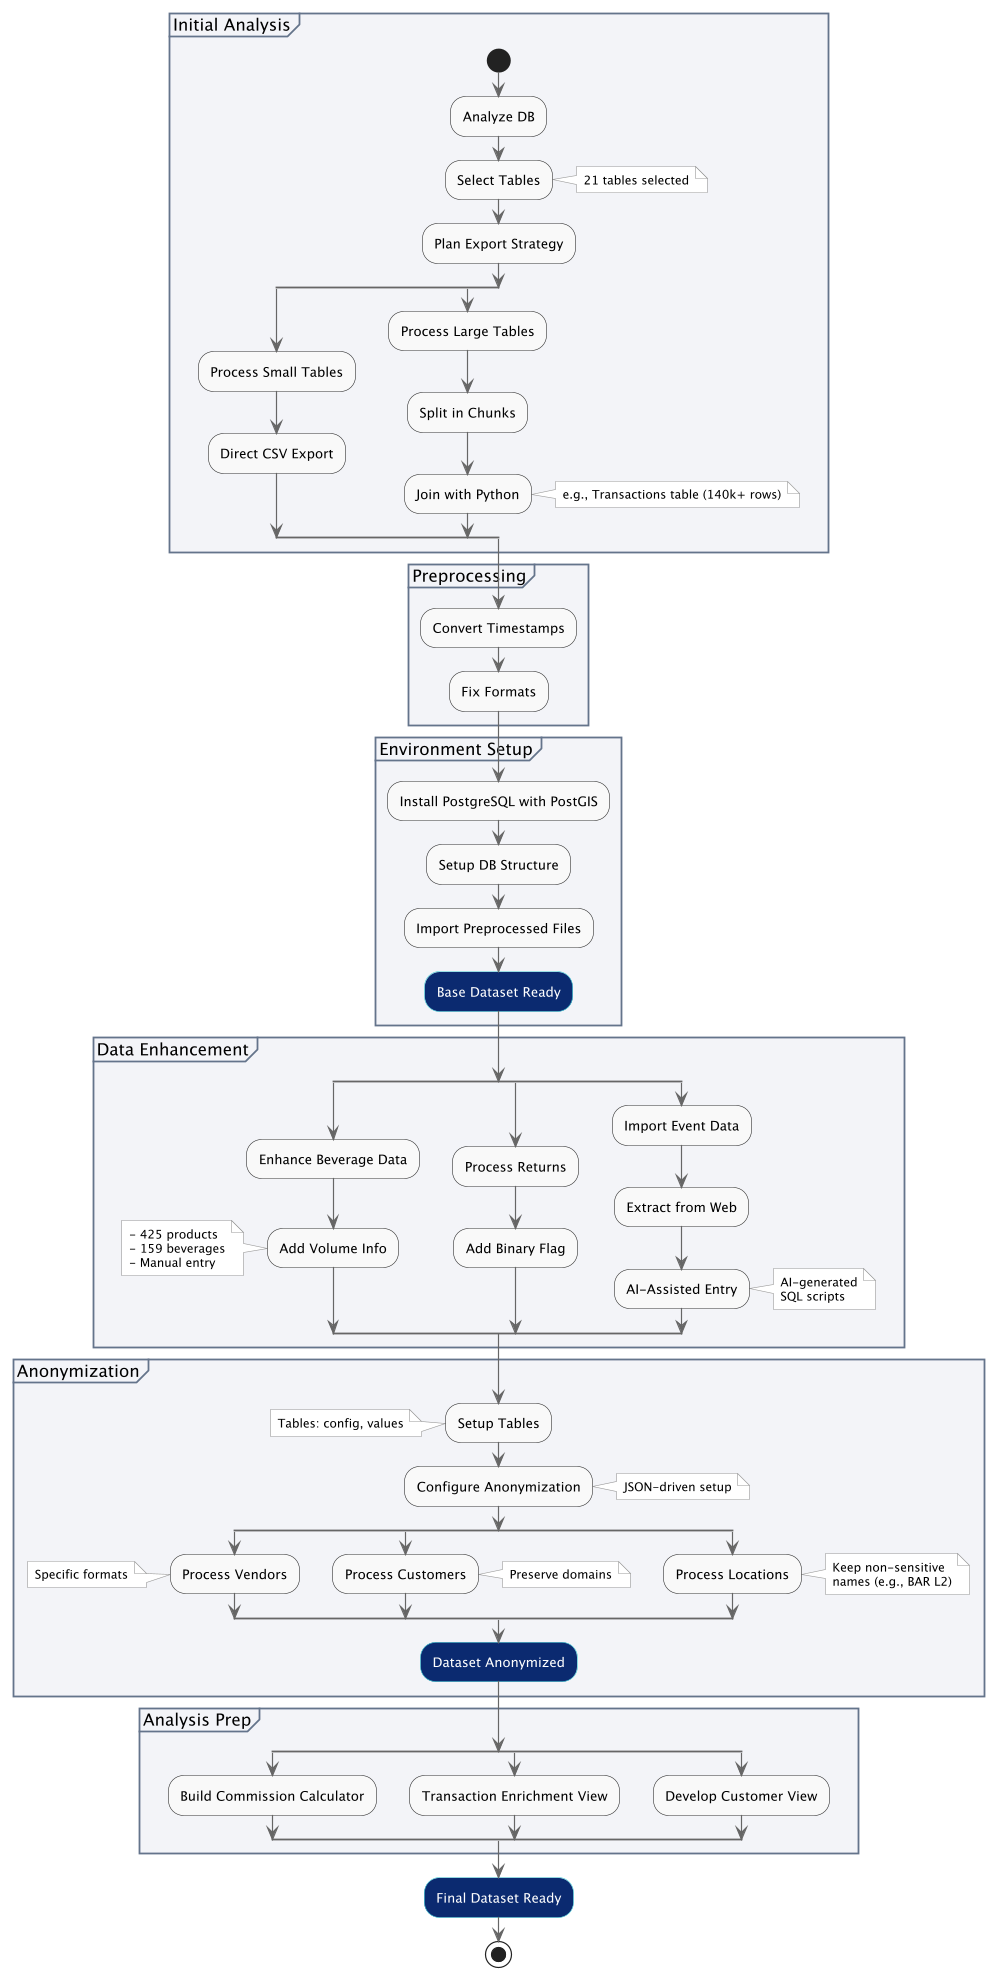
\includegraphics[width=0.8\textwidth]{\ThesisFigures/diagrams/kdd-workflow}
	\caption{Knowledge Data Discovery workflow diagram.}
	\label{fig:data-methodology-diagram}
\end{figure}

